\section{The Predator/Prey Example}
\label{section:the-predator-prey-example}

The predator/prey domain is an appropriate multi-agent example that has successfully been studied in a variety of instantiations. It does not serve as a complex real world domain, but as a test scenario for demonstrating and evaluating manifold research ideas. Introduced by \cite{BJD86}, researchers have investigated different instantiations of its original formulation in the context of different application areas \cite{SV00}. 

Both, predator and prey, typically can move into four different directions -- north, east, south, and west. Mostly, predators follow a capturing strategy as a goal, while the prey randomly moves or stays still with a certain probability in order to simulate slower movements than the predators. A variation is that the prey moves faster than the predators. In this case, a strategic collaborative effort is required by the predators. An active escaping strategy, where the prey adapts and learns its behavior, may also be possible.

% Worlds with other shapes as spaces (e.\,g., squares) or continuous/toroidal worlds without edges (predators and prey can move off one end of the world and come back on another end) are possible. 

% The predators try to capture the prey in such a way that the prey cannot move to an unoccupied position. If the grid world has edges, it might be possible that fewer than four predators can catch the prey by surrounding the prey against an edge of obstacles or in a corner of the world. Other parameters of the predator/prey domain are: Do the agents move simultaneously or successively -- one after the other? Is the local view of an agent limited or does an agent see the whole environment? And last, but not least, is direct communication between the agents allowed?

While predators and prey(s) have limited actions and follow well defined objectives, the predator/prey domain is simple to understand, easy to implement, and flexible enough to demonstrate a range of different scenarios, which have been emerged over the past decades. % The general approach of the predator/prey example, the possibility to customise and adopt the scenario to manifold applications, or the wide\-spread experience that is documented, not only in multi-agent literature, result in the assumption that the predator/prey example can be used as a valid and flexible testbed for technical OC scenarios.

Here, a simple implementation of the predator/prey scenario is examined, where the predators fulfil a cooperative observation task and are rewarded for just being very close to the prey. Thus, it is not necessary to surround and catch the prey, the predators try to observe the prey as long as possible. The overall scenario settings are described in Section~\ref{subsection:scenario-settings} followed by a detailed description of the investigated obstacle configurations in Section~\ref{subsection:scenario-obstacle}. % Putting all together the properties of the scenario are then compared to the properties of environments without the Markov property (see Section~\ref{subsection:scenario-classification}) and then classified according to the results of the discussion in Section~\ref{subsection:non-markov-environments}.

\subsection{Scenario Settings}
\label{subsection:scenario-settings}

The different XCS implementations are tested in a simple predator/prey scenario on a discrete, quadratic, and toroidal world consisting of $16 \times 16$ squares. One non-learning prey randomly moves over the field. % Eight adaptive predators do not follow a catching strategy, but cooperatively have to learn to keep the prey under observation. 
Eight adaptive predators follow an observation strategy. I.\,e., they cooperatively have to learn to keep the prey under observation. Thereby, every predator possesses its own XCS instance. 

A cell of the two-dimensional grid-world can only be occupied by one agent. The quality of the observation task is determined by the amount of time any predator has the prey in its observation range. It is calculated by averaging the qualities of 100 experiments, each consisting of 10 runs. In detail, each run consists of 2\,000 steps, after which the scenario is reset. The individual learning experiences of the agents are saved between each run, but not between each experiment.

In each time step, each predator can only move to one of the four neighboring fields, while the prey can move two fields, which allows for a faster movement. In addition, there are obstacles on the field and any movement to an occupied field fails (without any further consequences). Both, the prey and the predators, have 24 binary sensors that can sense their close environment, but their lines of sight can be blocked by objects. Half of the sensors can detect objects, which are two fields away, while the other half can detect objects up to five fields away, as depicted in Figure~\ref{figure:sight-directions}. % The 12 sensors for each sight range are for the four directions and the three types of objects (prey, other agents, and obstacles). An example of a resulting sensor data string is shown in Figure~\ref{figure:example-string}.
Thus, 12 binary-coded sensors are used for each sight range to encode every possible situation, as shown in Figure~\ref{figure:example-string}. Three bits are used to characterize a specific situation (prey, other predators, and obstacles) for each direction (north, east, south, and west). 

\begin{figure}[ht]
	\subfigure[Sight range]{
  	\label{figure:sight-range}
		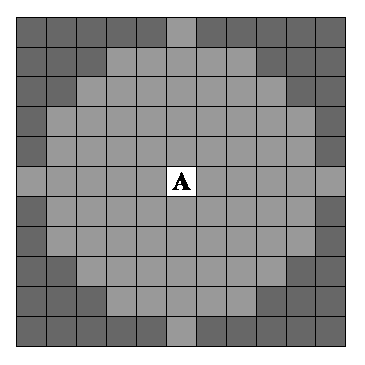
\includegraphics[height=2.55cm]{sight_range.eps}
  }\hfill
  \subfigure[Observation range]{
  	\label{figure:observation-range}
  	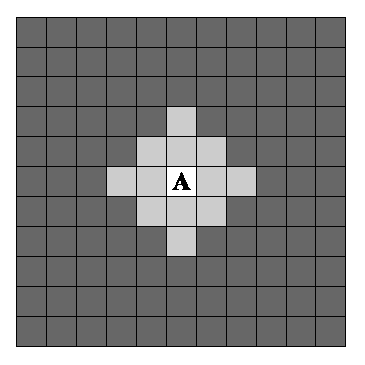
\includegraphics[height=2.55cm]{observation_range.eps}
  }\hfill
  \subfigure[Example situation]{ % with an agent, trees and food/prey]{
  	\label{figure:example-sight-observation}
  	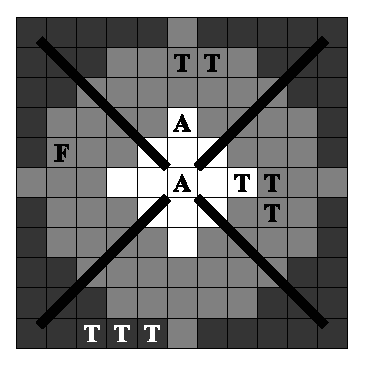
\includegraphics[height=2.55cm]{example_sight_observation.eps}
  }
  \caption{\mathversion{bold}Sensor ranges of individual agents and a example situation: Obstacles/trees are marked with $T$, prey/food is marked with $F$, predators/agents are marked with $A$, and the observation and sight ranges are marked with light grey and grey color, respectively. Areas, which are out of sight of any predator, are marked with dark grey color.}
  \label{figure:sight-directions}
\end{figure}

\begin{figure}[ht]
	\centerline{
		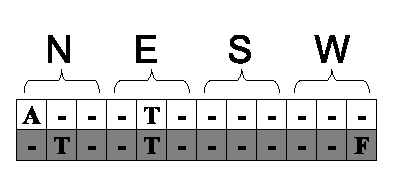
\includegraphics[width=0.2\textwidth]{example_string.eps}
	}
	\caption{\mathversion{bold}Matching sensor data string for the example, as depicted in Figure~\ref{figure:example-sight-observation}}
	\label{figure:example-string}
\end{figure}

% ANDERE ABBILDUNG UND EIN BEISPIEL ERGAENZEN

The simulation is conducted in discrete time. At every time step, the prey and the predators gather sensor data and decide their next actions. Then, all actions of all agents are executed in a random sequence. Since the prey can move two fields, it gathers new sensor data after the first step. If the prey is surrounded by predators in all four neighboring directions, it will jump to a random free field nearby, which basically means a restart of the simulation. Experiments have shown that this random jumping strategy only happens very seldom, i.\,e., it does not significantly alter the simulation results.

\subsection{Scenario Configurations}
\label{subsection:scenario-obstacle}

Three different configurations of obstacles (trees) and star\-ting positions of prey and predators have thoroughly been tested. 

\begin{figure}[ht]
	\subfigure[\emph{Pillar sce\-nar\-io}]{
  	\label{figure:pillar-scenario}
		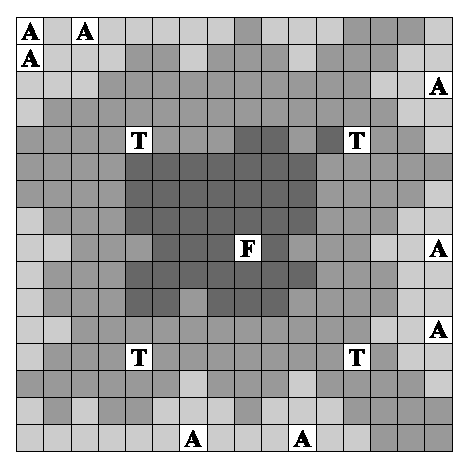
\includegraphics[height=2.55cm]{pillar_scenario.eps}
  }\hfill
  \subfigure[\emph{Random sce\-nar\-io}]{
  	\label{figure:random-scenario}
  	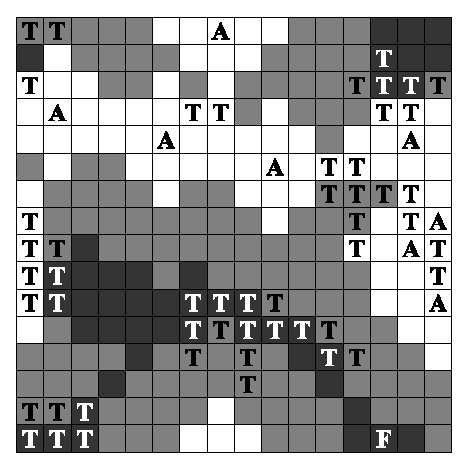
\includegraphics[height=2.55cm]{random_scenario.eps}
  }\hfill
  \subfigure[\emph{Difficult sce\-nar\-io}]{
  	\label{figure:difficult-scenario}
  	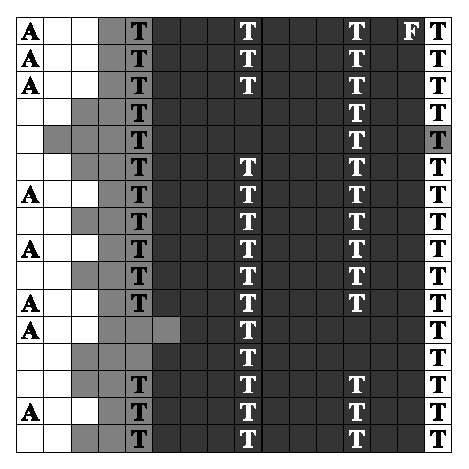
\includegraphics[height=2.55cm]{difficult_scenario.eps}
  }
  \caption{\mathversion{bold}Sample start configurations for the three different scenarios: Obstacles/trees are marked with $T$, prey/food is marked with $F$, predators/agents are marked with $A$, and the observation and sight ranges are marked with light grey and grey color, respectively. Areas, which are out of sight of any predator, are marked with dark grey color.}
  \label{figure:scenarios}
\end{figure}

In the \emph{pillar scenario} (see Figure~\ref{figure:pillar-scenario}), four obstacles are arranged in equal distance to each other, the prey starts in the middle of the whole field, and the predators start randomly positioned along the borders. The idea of this scenario has been to use a minimal number of obstacles while still giving the agents some points of orientation.

In the second scenario, the \emph{random scenario} (see Figure~\ref{figure:random-scenario}), several obstacles are randomly distributed on the field with a certain tendency to build connected structures. 

In both scenarios, the \emph{pillar scenario} and the \emph{random scenario}, two kinds of prey implementations have been tested. The first one tries to move away from predators (\emph{predator-evading prey}) while the second one tries to evade collisions with obstacles  (\emph{obstacle-evading prey}). Both types of preys move randomly.  walk strategy as well, but tries to evade collisions with obstacles.

The third scenario, the \emph{difficult scenario} (see Figure~\ref{figure:difficult-scenario}), provides some kind of a labyrinth with several walls and small openings. Predators start on the left and have to find the openings that lead them into the direction of the prey, while the prey only stays in the area on the right and continuously moves northward for two fields (or will jump to a free field nearby, if the direct path is blocked in northern direction). As the prey ignores sensory information it will be referred to as \emph{blind prey}.


\subsection{Classification of the Scenario}
\label{subsection:scenario-classification}

As described in Section~\ref{subsection:non-markov-environments}, environments can be classified as a MDP, a POMDP, or a NOMDP. The main characteristics of the predator/prey scenario, which is here investigated, could be summarized as follows:

\begin{enumerate*}
	\item An agent has only access to local information,
	\item the whole field usually consists of open areas with randomly placed obstacles,
	\item each agent has an internal state unknown to others,
	\item the scenario is dynamic (agents act in parallel),
	\item the agents (i.\,e., the predators) share and cooperatively contribute to a glo\-bal observation task, and
	% \item the scenario runs continuously.
	\item the global observation task forces continuous agents' activities.  
\end{enumerate*}

It is obvious that the three scenarios, as intended in Figure~\ref{figure:scenarios}, constitute being no MDPs, since sensory information is limited (1, 3) and different positions share the same sensory configuration (2). Moreover, adding the capability of storing information in a memory would not restore the Markov property (4), as proposed in \cite{Lan98,LW00}. This let us conclude that the scenarios could not be any POMDPs. Finally, this also remains that the scenarios have to be NOMDPs. 

Additionally, if each predator tries to learn its cooperative behavior using an XCS, a clearly defined (local) goal (5) will be needed to generate payoffs when agents have reached their goals. Furthermore, a typical multi-step scenario will be restarted, if an agent has reached its goal. But, the observation task is a continuous task (6). % In addition, special care is needed when applying XCS as is no clear local goal (5) and the scenario is not restarted when reaching the global goal (6). 
To conclude, a different approach is needed. Thus, a modified multi-step XCS variant is introduced in the following that can properly handle these issues.

In XCS literature, NOMDP environments are discussed in \cite{Miyazaki2,TTS01}. There, the issue of non observability is either investigated by a very simplified scenario with only two agents or by using complex communication and centralized organization mechanisms, where all agents share and contribute to a global LCS with global information. Both approaches seems not applicable here, since the three scenarios focus on more than two agents and (global) communication between the predators is not intended. Thus, new mechanisms are required to learn this % cooperative 
collaborative and dynamic observation task using the XCS algorithm. The most important step to solve this problem is the design of an adequate reward function, which is discussed in the following section.
